%! Author = chtompki
%! Date = 1/14/26
\documentclass[10pt]{amsart}
% Default margins are too wide all the way around. I reset them here
\setlength{\hoffset}{-.75in}
\setlength{\textwidth}{6.5in}
\setlength{\voffset}{-.5in}
\setlength{\textheight}{9.0in}
\usepackage{amsmath}
\usepackage{amssymb}
\usepackage{amsthm}
\usepackage{lmodern}
\usepackage{microtype}
\usepackage{enumitem}
\usepackage{setspace}
\usepackage{graphicx}
\usepackage{hyperref}
\usepackage{tikz}
\usepackage{listings}
\usepackage{pgfplots}
\pgfplotsset{compat=1.18}
\usepgfplotslibrary{groupplots}


\newenvironment{solution}
{\begin{proof}[Solution]}
{\end{proof}}

\NewDocumentCommand{\vitem}{v}{%
    \item[\texttt{#1}]%
}

\newcommand{\slopeelement}[3]{%
    \pgfmathsetmacro{\slopeDX}{0.14/sqrt(1+(#3)^2)}%
    \pgfmathsetmacro{\slopeDY}{(#3)*\slopeDX}%
    \pgfmathsetmacro{\slopeXA}{(#1)-\slopeDX}%
    \pgfmathsetmacro{\slopeYA}{(#2)-\slopeDY}%
    \pgfmathsetmacro{\slopeXB}{(#1)+\slopeDX}%
    \pgfmathsetmacro{\slopeYB}{(#2)+\slopeDY}%
    \edef\slopecommand{%
        \noexpand\draw[gray,thin]
        (axis cs:\slopeXA,\slopeYA)
        --
        (axis cs:\slopeXB,\slopeYB);%
    }%
    \slopecommand
}

\title{Dynamical Systems\\Problem Set 2}
\author{Rob Tompkins}
\date{\today}

\begin{document}
    \maketitle
    \date{\today}
    \begin{onehalfspace}
        We begin by noting that all of the files referenced in this document are available at: \\
        \underline{https://github.com/chtompki/MathFall2026/tree/main/DynamicalSystems/ProblemSet2}

        The next exercises (3.4.5, 3.5.7, and 3.4.9) are designed to test your ability to distinguish among the various
        types of bifurcations --- its easy to confuse them!
        In each case, fine the values of $r$ at which bifurcations occur, and classify those as: saddle-node,
        transcritical, supercritical pitchfork, or subcritical pitchfork.
        Finally sketch the bifurcation diagram of fixed points $x^*$ vs $r$.

        \noindent\textbf{3.4.5} $\dot{x} = r - 3x^2$

        \begin{solution}
        \end{solution}

        \noindent\textbf{3.4.7} $\dot{x} = 5 - re^{-x^2}$

        \begin{solution}
        \end{solution}

        \noindent\textbf{3.4.9} $\dot{x} = x = \tanh{(rx)}$

        \begin{solution}
        \end{solution}

        \noindent\textbf{3.4.11} (An interesting bifurcation diagram) Consider $\dot{x} = rx - \sin{(x)}$
        \begin{itemize}
            \item[a)] For the case $r = 0$, find and classify all the fixed points, and sketch the vector field.
            \item[b)] Show that when $r > 1$, there is only one fixed point.
            What kind of fixed point is it?
            \item[c)] As $r$ decreases from $\infty$ to $0$, classify \emph{all} the bifurcations that occur.
            \item[d)] For $0 < r \ll 1$, find an approximate formula for all values of $r$ at which bifurcations occur.
            \item[e)] Now classify all the bifurcations that occur as $r$ decreases from $0$ to $-\infty$.
            \item[f)] Plot the bifurcation diagram for $-\infty < r < \infty$, and indicate the stability of the various
            fixed points.
        \end{itemize}

        \begin{solution}
        \end{solution}

        \noindent\textbf{3.4.14} (Subcritical pitchfork) Consider the system $\dot{x} = rx + x^3 -x^5$, which
        exhibits a subcritical pitchfork bifurcation.
        \begin{itemize}
            \item[a)] Find algebraic expressions for the all the fixed points at $r$ varies.
            \item[b)] Sketch the vector fields as $r$ varies.
            Be sure to indicate all the fixed points and their stability.
            \item[c)] Calculate $r_s$, the parameter value at which the nonzero fixed points are born in a saddle-node
            bifurcation.
        \end{itemize}

        \begin{solution}
        \end{solution}

        \noindent\textbf{3.4.16} (Potentials) In parts (a)-(c) let $V(x)$ be the potential, in the sense that
        $\dot{x} = -dV/dx$.
        Sketch the potential as a function of $r$.
        Show all qualitatively different cases including bifurcation values of $r$.
        \begin{itemize}
            \item[a)] (Saddle-node) $\dot{x} = r - x^2$
            \item[b)] (Transcritical) $\dot{x} = rx - x^2$
            \item[c)] (Subcritical pitchfork) $\dot{x} = rx + x^3 - x^5$.
        \end{itemize}

        \begin{solution}
        \end{solution}

        \noindent\textbf{3.5.4} (Bead on a horizontal wire) A bead of mass $m$  is constrained to slide along
        a straight horizontal wire.
        A spring of relaxed length $L_0$ and spring constant $k$ is attached to the mass and to a support point
        distance $h$ from the wire given in Figure \ref{figure1} below.

        \begin{figure}[htbp]
            \centering
            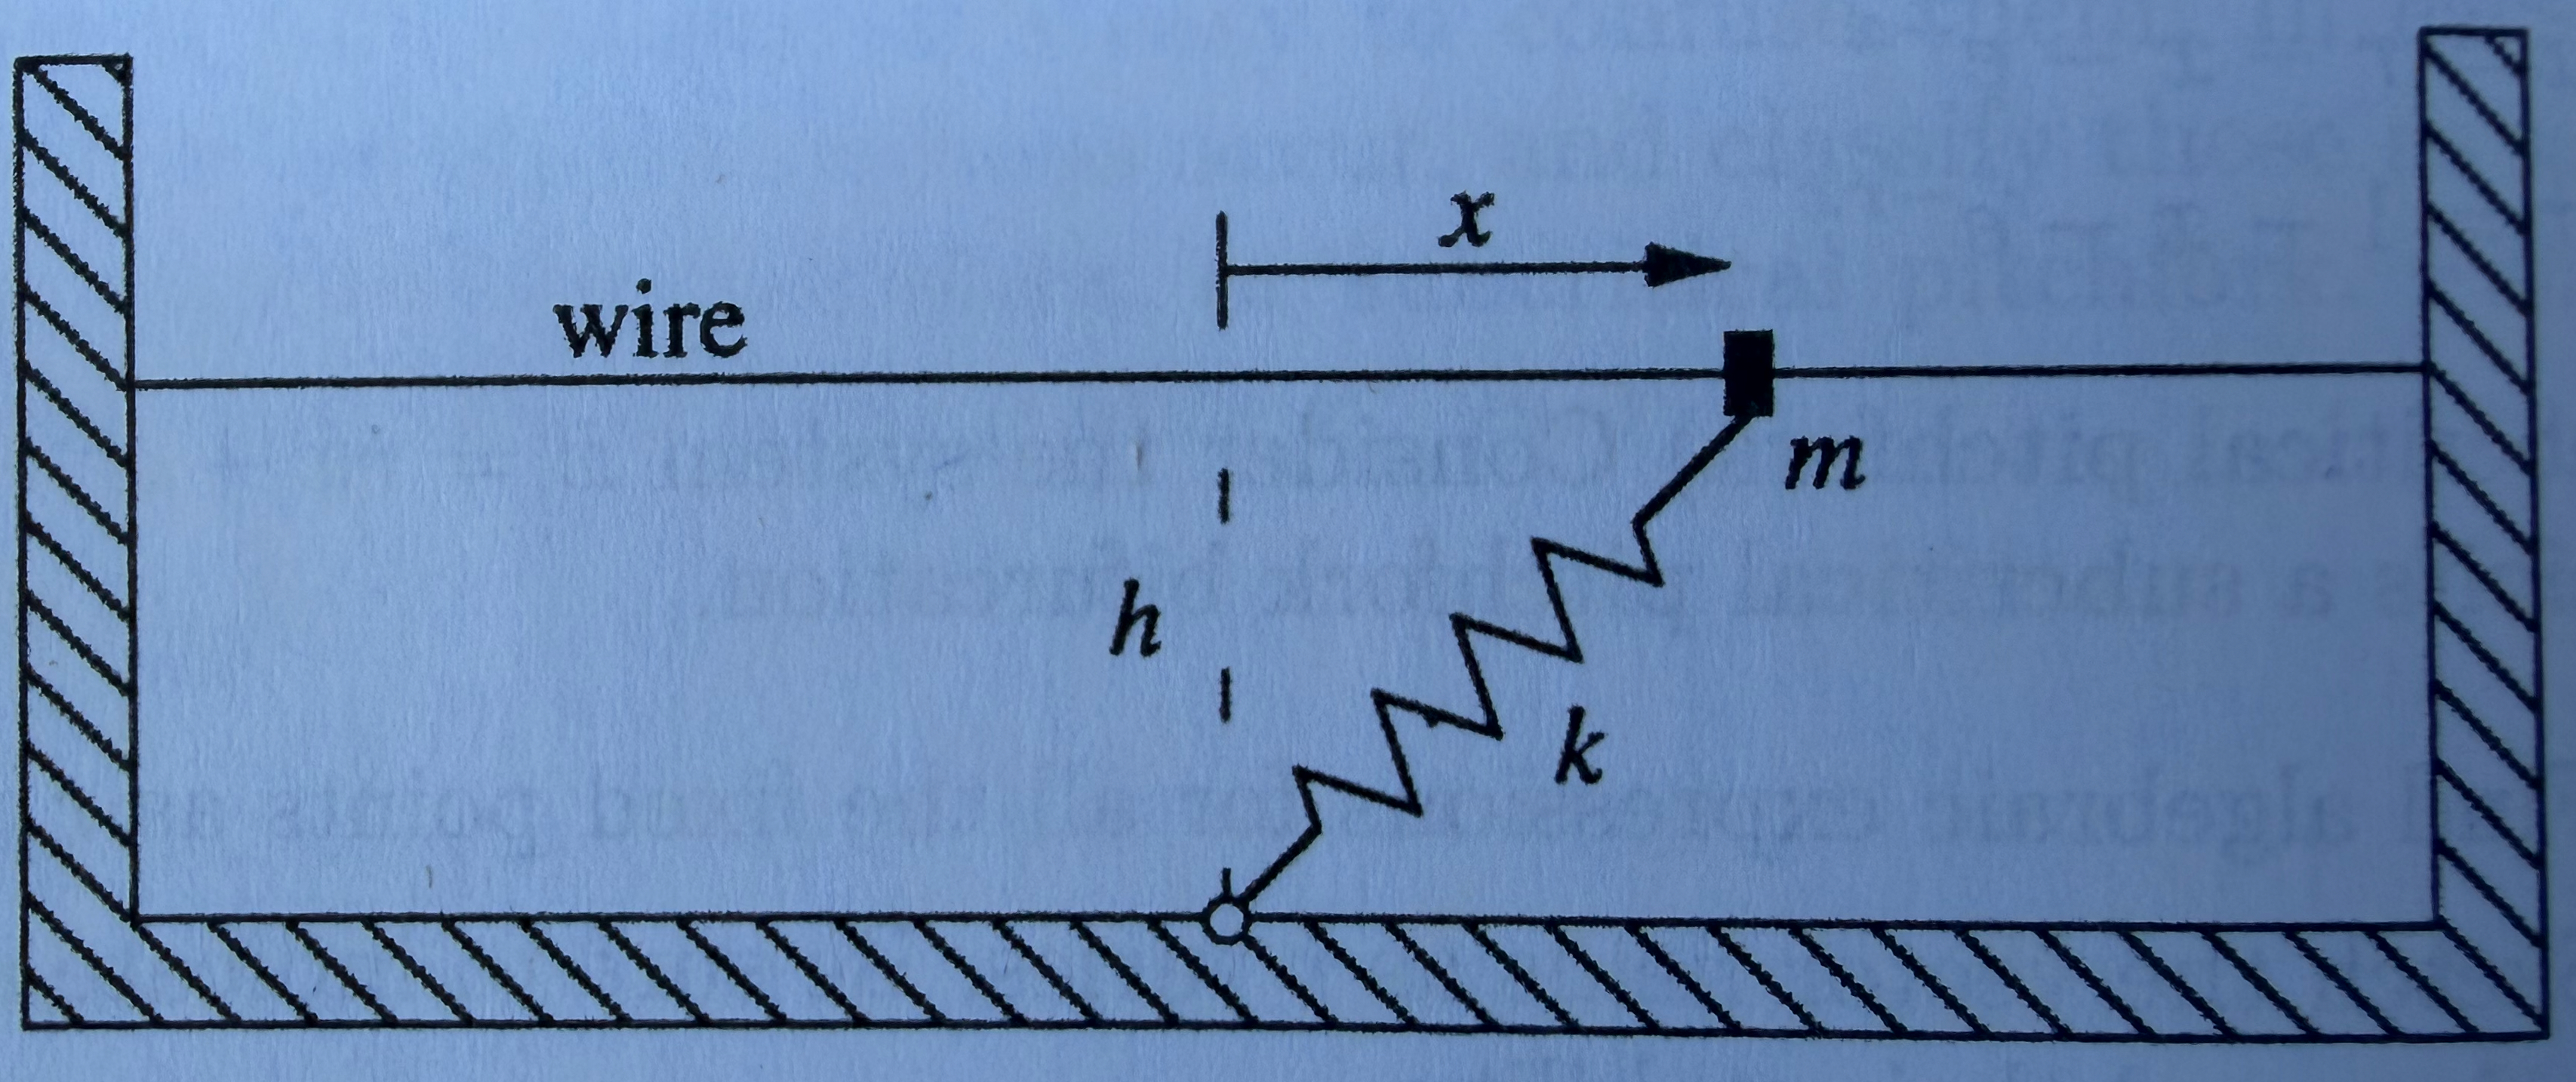
\includegraphics[width=\textwidth]{figure1.jpeg}
            \caption{}
            \label{figure1}
        \end{figure}

        \noindent Finally suppose that the motion of the bead is opposed by a viscous damping force $b\dot{x}$.
        \begin{itemize}
            \item[a)] Write Newton's law for the motion of the fixed bead.
            \item[b)] Find all possible equilibria, i.e. fixed points, as functions of $k$, $h$, $m$, $b$, and $L_0$.
            \item[c)] Suppose $m = 0$.
            Classify the stability of all the fixed points, and draw a bifurcation diagram.
            \item[d)] If $m\neq 0$, how small must $m$ be, to be considered negligible?
            In what sense is it negligible?
        \end{itemize}

        \begin{solution}
        \end{solution}

        \noindent\textbf{3.6.2} (Imperfect transcritical bifurcation) Consider the system $\dot{x} = h + rx - x^2$.
        When $h = 0$, this system undergoes a transcritical bifurcation at $r = 0$.
        Our goal is to see how the bifurcation diagram of $x^*$ vs. $r$ is affected by the imperfection parameter $h$.
        \begin{itemize}
            \item[a)] Plot the bifurcation diagram for $\dot{x} = h + rx - x^2$, for $h < 0$, $h = 0$, and $h > 0$.
            \item[b)] Sketch the regions in the $(r,h)$ plane that correspond to qualitatively different vector fields,
            and identify the bifurcation that occur on the boundaries of those regions.
            \item[c)] Plot the potential $V(x)$ corresponding to all the different regions in the $(r,h)$ plane.
        \end{itemize}

        \begin{solution}
        \end{solution}

        \noindent\textbf{3.7.5} (A biochemical switch) Zebra stripes and butterfly wing patterns are two of the most
        spectacular examples of biological pattern formation.
        Explaining the development of these patterns is on of the outstanding problems of Biology; see Murray (2003)
        for an excellent review.

        As one ingredient in a model of pattern formation, Lewis et al. (1977) considered a simple example of a
        biochemical switch, in which a gene $G$ is activated by a biochemical signal substance $S$.
        For example, the gene may normally be inactive but can be ``switched on'' to produce a pigment or other gene
        product when concentration of $S$ exceeds a certain threshold.
        Let $g(t)$ denote the concentration of the gene product, and assume that the concentration $s_0$ of $S$ is
        fixed.
        The model is
        \[
            \dot{g} = k_1 s_0 - k_2 g + \frac{k_3 g^2}{k_4^2 + g^2},
        \]
        where $k$'s are positive constants.
        The production of $g$ is stimulated by $s_0$ at rate $k_1$, and by an \emph{autocatalytic} (positive feedback)
        process, modeled by the non-linear term.
        There is also a linear degradation of $g$ at a rate $k_2$.
        \begin{itemize}
            \item[a)] Show that the system can be put in the dimensionless form
            \[
                \frac{dx}{d\tau} = s - rx + \frac{x^2}{1+x^2},
            \]
            where $r > 0$ and $s\ge 0$ are dimensionless groups.
            \item[b)] Show that if $s = 0$, there are two positibe fixed points $x^*$ if $r < r_c$, where $r_c$ is to
            be determined.
            \item[c)] Assume that initially there is no gene product, i.e. $g(0) = 0$, ad suppose $s$ is slowly
            increased from $0$ (the activating signal is turned on); what happens to $g(t)$?
            What happens if $s$ then goes back to zero?
            Does the gene turn off again?
            \item[d)] Find parametric equations for the bifurcation curves in $(r, s)$ space, and classify
            the bifurcations that occur.
            \item[e)] Compute a quantitatively accurate plot of the stability diagram in $(r, s)$ space.
        \end{itemize}
        For further discussion of this model, see Lewis et al. (1977); Edelstein-Kishet (1988); Section 7.5; or
        Murray (2002), Chapter 6.

        \begin{solution}
        \end{solution}

        \noindent\textbf{5.1.10} (Attracting and Liapunov stable) here are the official definitions of various
        types of stability.
        Consider a fixed point $\mathbf{x^*}$ of a system $\mathbf{\dot{x} = f(x)}$.

        \noindent We say that $\mathbf{x^*}$ is \textbf{\emph{attracting}} if there is a $\delta >0$ such that
        $\lim\limits_{t\rightarrow\infty} x(t) = \mathbf{x^*}$ whenever $\|\mathbf{x}(0) - \mathbf{x^*}\| < \delta$
        within a distance of $\delta$ to $\mathbf{x^*}$ is guaranteed to converge to $\mathbf{x^*}$ \emph{eventually}.
        As shown schematically in Figure \ref{figure2}, trajectories that start nearby are allowed to stray from
        $\mathbf{x^*}$ in the short run, but the must approach $\mathbf{x^*}$ in the long run.

        \noindent In contrast, Liapunov stability requires that nearby trajectories remain close for \emph{all} time.
        We sayt that $\mathbf{x^*}$ is \textbf{\emph{Liapunov stable}} if for each $\varepsilon > 0$ there is a
        $\delta > 0$ such that $\|\mathbf{x}(t) - \mathbf{x^*}\| < \varepsilon$ whenever $t \ge 0$ and
        $\|\mathbf{x}(0) - \mathbf{x^*}\| < \delta$.
        Thus, trajectories that start within $\delta$ of $\mathbf{x^*}$ remain within $\varepsilon$ of $\mathbf{x^*}$
        for all positive time.
        Figure \ref{figure2} gives a good example of this
        \begin{figure}[htbp]
            \centering
            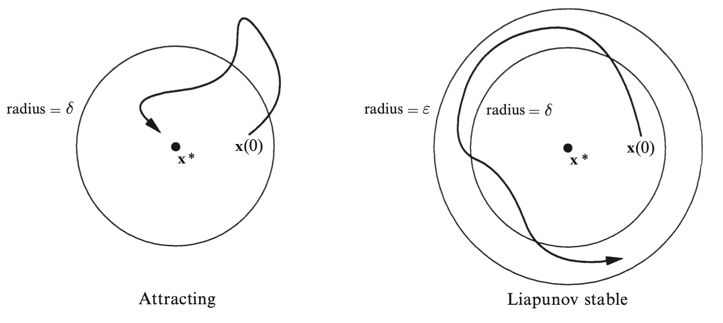
\includegraphics[width=\textwidth]{figure2.png}
            \caption{}
            \label{figure2}
        \end{figure}
        Finally $\mathbf{x^*}$ is \textbf{\emph{asymptotically stable}} if it is both attracting and Liapunov stable.

        \noindent For each of the following systems, decide whether the origin is attracting, Liapunov stable,
        asymptotically stable, or none of the above.
        \begin{itemize}
            \item[a)] $\dot{x} = y$, $\dot{y} = -4x$
            \item[b)] $\dot{x} = 2y$, $\dot{y} = x$
            \item[c)] $\dot{x} = 0$, $\dot{y} = x$
            \item[d)] $\dot{x} = 0$, $\dot{y} = -y$
            \item[e)] $\dot{x} = -x$, $\dot{y} = -5y$
            \item[f)] $\dot{x} = x$, $\dot{y} = y$
        \end{itemize}

        \begin{solution}
        \end{solution}

        \noindent\textbf{5.2.1} Consider the system $\dot{x} = 4x - y$, $\dot{y} = 2x + y$.
        \begin{itemize}
            \item[a)] Write the system as $\mathbf{\dot{x}} = A \mathbf{x}$.
            Show that the characteristic equation is $\lambda^2 - 5\lambda + 6 = 0$,
            and find the eigenvalues and eigenvectors of $A$.
            \item[b)] Find the general solution of the system.
            \item[c)] Classify the fixed point at the origin.
            \item[d)] Solve the system subject ot the initial condition $(x_0, y_0) = (3, 4)$.
        \end{itemize}

        \begin{solution}
        \end{solution}

        \noindent\textbf{5.2.6} Plot the phase portrait and classify the fixed point of the following
        linear systems.
        If the eigenvectors are real, indicate them in your sketch.
        \begin{eqnarray*}
            \dot{x} & = & -3x + 2y \\
            \dot{y} & = & x - 2y
        \end{eqnarray*}

        \begin{solution}
        \end{solution}

    \end{onehalfspace}
\end{document}